The goal of this chapter is to combine the techniques we presented in Chapters~\ref{chapter:detection},\ref{chapter:fruit_counting},\ref{chapter:sfm} and \ref{chapter:merge_both} to compute the aggregate fruit count for the captured portion of a tree row. We have already presented methods to estimate the underlying scene geometry and camera motion from both sides of a tree row. In this chapter, we will utilize them to track fruit in consecutive frames, eliminate fruit on the ground and other tree rows and alleviate double-counting owing to fruit visible from both sides of a row. 


To be more specific, in chapter~\ref{chapter:sfm}, we presented a method to recover underlying scene geometry from footage captured from a single side of a tree row. Here, we present techniques for tracking fruit using these reconstructions from single sides. We also present a baseline tracking method using homographies which does not require Structure from motion(SfM). We perform comparisons between the two strategies demonstrating the superiority of incremental SfM method. We also remove fruit on the ground plane and other rows with the help of the reconstructions.

Likewise, in Chapter~\ref{chapter:merge_both}, we presented techniques for merging independent reconstructions from both sides of a tree row to obtain a coherent geometric representation. In this chapter, we present the techniques to eliminate double-counting owing to fruit visible from both sides using the merged models.


The rest of the chapter is organized as follows. We study single-side tracking in Section~\ref{sec:track_single}. In section~\ref{sec:track_both} we present a method for eliminating fruit visible from both sides. We present complete yield estimation results in Section~\ref{sec:track_exp}. Finally, we conclude in Section~\ref{sec:track_conc} with current limitations and possible ways to solve them. We start with single-side tracking in the next section.




\section{Tracking Fruit from Single Side of a Row}\label{sec:track_single}
To obtain accurate fruit count for each cluster we merge the counts from different frames. For this purpose, we need to establish the correspondence between the clusters across multiple frames by utilizing the estimated camera motion. In this section, we present two different approaches to accomplishing this task. First, we present a method for tracking that assumes that the underlying scene is mostly planar and approximates camera motion by homographies. Second, we present a method that performs incremental SfM and tracks the fruit using the reconstructed scene structure and computed the camera poses.

\subsection{Tracking by Pairwise Homography}\label{sec:merge_homography}
As our camera viewing direction does not change much, and if we assume that the scene is roughly planar, we can model the camera motion between consecutive frames by pairwise homography \cite{eshel2008homography}. The homography between frames is estimated by matching SIFT \cite{sift} features above the ground. Using homography we will keep track of the boxes generated by the connected component analysis across the entire image sequence (Fig.~\ref{fig:trackcluster}).

\begin{figure}[!hbpt]
        \centering
            \includegraphics[width =0.99\textwidth]{figures/map_yield/clusterTrack_.pdf}           
   \caption[Tracking fruit over sequence of frames]{Tracking an apple cluster over $31$ frames. For clarity only $13$ frames with significant changes are shown. The arrows indicate the direction of the views from start to end.}
   \label{fig:trackcluster}
\end{figure}

Let $b^1_1, b^1_2, \ldots b^1_m$ be the bounding boxes generated by connected component analysis for frame $1$. Let the apple count for each of these boxes be $c^1_1, c^1_2, \ldots c^1_m$ (computed by the counting method). When we find a bounding box for the first time we initialize a counting list that contains computed counts from the first frame.

Now for frame $2$, let the bounding boxes be $b^{2}_1, b^{2}_2, \ldots b^{2}_n$ and the counts be $c^{2}_1, c^{2}_2, \ldots c^{2}_n$. Let the homography that maps frame $1$ to frame $2$ be $^2 H_{1}$. We propagate all the bounding boxes in frame $1$ to frame $2$ using $^2 H_{1}$. This is executed by multiplying the center of each bounding box with $^2 H_{1}$. Next, we check the overlap between these propagated bounding boxes and the original bounding boxes on frame $2$. If the overlap is more than $10\%$ we assume that these bounding boxes correspond to the same cluster. We will add the apple count to the list initialized previously using the following rules:

\begin{itemize}

\item When a bounding box in the current frame does not overlap with any of the propagated bounding boxes, a new counting list for this box is initialized with the current count.


\item When only one bounding box in the current frame overlaps with a propagated bounding box, the count from the bounding box in the current frame is added to the counting list for the propagated box

\item Otherwise, when two or more bounding boxes overlap with a bounding box from the previous frame, their counts are added to obtain the total count to be recorded in the list. To have a better understanding of this rule, we consider the following scenario: Let $b^2_1, b^2_3$ be overlapping with $b^1_1$. Prior to frame $2$ the counting list of $b^1_1$, $c_{b^1_1}$ had only one entry, $c^1_1$. As there is overlap, a new entry will be inserted. This new entry is $c'^2_1 = c^{2}_1 + c^{2}_3$.

\item The overlapping bounding boxes are unioned to obtain a new bounding box covering all of them. These new bounding boxes will be propagated to the next frame.


\end{itemize}


\begin{figure}[!hbpt]

        \centering        
            \includegraphics[width =0.90\textwidth]{figures/map_yield/mergeApples_.pdf}         
        
   %\caption{An example from the GMM counting method.
  
  \caption[Tracking a fruit cluster across frames by homography]{Tracking fruit clusters across frames. We keep track of the corresponding bounding boxes generated connected component analysis across multiple frames using homography. The count for every box from different frames is recorded throughout the entire video. In this example, $box_1$ appeared in frame $1,3, \ldots ,8$ and the counts for each of these frames $C_1,C_3 \ldots C_8$ were recorded. The median counts for each box are reported as the final output of the counting method.}
   \label{fig:mergecount}
\end{figure}    

At the end of the image sequence, we have a set of unique boxes with count lists. We compute the median for each of the boxes and the sum of these are reported as the total count (Fig.~\ref{fig:mergecount}).




\subsection{Tracking from Single-side 3D Reconstructions}\label{subsec:tracking} 
Modern orchards are moving toward settings where fruit is essentially growing on a 2D plane. In such cases, homographies provide a good approximation as we are looking at a planar scene. However, in traditional orchards, this is not the case. For these instances, we have to utilize the full camera motion estimated by the method described in chapter~\ref{chapter:sfm}.


Given an input image (Fig.~\ref{fig:trackpipeline}(a)) we used the detection step to obtain a segmentation mask, containing only the fruit (Fig.~\ref{fig:trackpipeline}(b)). Afterward, we used Structure from Motion (SfM) to obtain a semi-dense 3D reconstruction of the trees (Fig.~\ref{fig:trackpipeline}(c)). However, the resulting point cloud does not have a one-to-one correspondence with the pixels in the images. To establish this correspondence, we projected the reconstructed point cloud to the camera frames (Fig.~\ref{fig:trackpipeline}(d)). We computed the intersection of the reprojected image and the binary mask to identify the 3D points belonging to the detected apples (Fig.~\ref{fig:trackpipeline}(e)). Subsequently, we performed a connected component analysis in 3D (Fig.~\ref{fig:trackpipeline}(f)). By using these connected components together with the estimated camera poses from SfM, we can reproject the outlines of these connected components onto an image series. These outlines provided us with a series of Region of Interest (RoI) that all show the same cluster of fruit (Fig.~\ref{fig:trackpipeline}(g)). A 3D cluster may appear in several frames (see Fig.~\ref{fig:trackpipeline}(g)). We chose the three frames with the highest amount of segmented apple pixels and reported the median count of these three frames as the fruit count for the cluster. 

\begin{figure}[!hbpt]
    \centering
    \def\svgwidth{\textwidth}
    \import{figures/map_yield/}{tracking_schematic.pdf_tex}\label{fig:track}
    \caption[Schematic overview of the fruit tracking and yield estimation pipeline.]{Schematic overview of the fruit tracking and yield estimation pipeline. (a) Input image; (b) Segmentation of the fruit; (c) 3D Reconstruction of a single side of the tree row; (d) Reprojection of fruit on 2D images; (e) Segmented pointcloud; (f) 3D connected components in 3D; (g) Tracked fruit clusters reprojected across multiple frames; (h) Fruit clusters visible from both sides of a tree row; (i) Elimination of double counting for fruit visible from both sides.}
    \label{fig:trackpipeline}
\end{figure}



\begin{figure}[!hbpt]
    \centering
    \def\svgwidth{\textwidth}
    \import{figures/map_yield/}{gpremoved.pdf_tex}\label{fig:gpremoved}
    \caption[Schematic overview of the removal of fruit on the ground and on trees in the background.]{Schematic overview of the removal of fruit on the ground and on trees in the background. (a) All Detections; (b) Mask for removing ground plane and fruit in the background; (c) Filtered detections}
    \label{fig:gp_removed}
\end{figure}

We removed the apples on the ground and trees in the background for all the single-side counts by using a computed 3D ground plane and depth masks. We performed these steps for both sides of the row. Fig.~\ref{fig:gp_removed} shows an overview of this process. 



\section{Merging Fruit Counts from Both Sides}\label{sec:track_both}
Detecting fruit and counting them in a per-frame manner, and tracking them from a single side are technically challenging tasks. However, these are only subproblems to the yield estimation task, which we ultimately want to solve. In this section, we combine all the information and compute the overall yield. 

We utilize the merged 3D reconstructions from the front- and backside of the tree row to eliminate double-counting of fruit that is visible from both sides. We used the algorithm described in Chapter~\ref{chapter:merge_both} to accomplish this task. We computed the intersection of the connected components from both sides (Fig.~\ref{fig:trackpipeline}(h)). Then, we computed the total counts by summing up the counts from all the connected components, computing the intersection area among them (among 1, 2,..., the total number of intersecting clusters) and adding/subtracting the weighted parts using the Inclusion-Exclusion principle~\cite{andreescu_inclusion-exclusion_2004} (Fig.~\ref{fig:trackpipeline}(i)). 





\section{Experiments}\label{sec:track_exp}
To evaluate yield estimation performance we arbitrarily chose three different sections of the orchard. We collected six videos from these four segments in 2016. These sections were annotated manually with bounding boxes to mark fruit locations. We also collected ground truth for the rows in question by collecting per tree yield and by measuring fruit diameters after harvest. These datasets are the same ones that were used for evaluating fruit detection, counting and merging scene geometry from both sides.

\subsection{Merging Counts Across Multiple Frames with Homography}

To verify the performance of the single-side tracking method, we utilize the manual annotations. We treat the manually annotated fruit as human perceived ground truth. Afterward, we track these fruit across frames using camera motion (3D camera poses) to avoid double counting and find the number of unique apples. The counts obtained in this manner are then compared to the counts from the homography based merging algorithm. We performed this evaluation by simply comparing the number of unique manually labeled apples obtained from homography to the number of unique apples obtained by utilizing full 3D camera motion. We found that across different datasets; using homography can lead to $8\%$ overcounting. Fig.~\ref{fig:countingtrack}(\subref{fig:trackHom}) shows these results. 
\begin{figure*}[!hbpt]
        \centering
        \begin{subfigure}[b]{\textwidth}\begin{subfigure}[b]{.49\textwidth}
                 \includegraphics[width=\textwidth]{figures/map_yield/trackingbyHomography_.pdf}
                 \caption{Evaluation of tracking by homography.}
                     \label{fig:trackHom}   
        \end{subfigure}\begin{subfigure}[b]{.49\textwidth}
                         \includegraphics[width=\textwidth]{figures/map_yield/datasetWiseCountingModel_.pdf}
                 \caption{Performance comparison of \supemph{semi-supervised} and \supemph{user-supervised} models for counting.}
                     \label{fig:dsetcountmodel}   
        \end{subfigure}
        \end{subfigure}       
   \caption[Effectiveness of tracking by homography and detection methods for counting.]{Evaluating the performance of the counting algorithm along with tracking. The figure on left shows the percentage of overcounting due to using homography for tracking (up to $8\%$). Fig. on the right shows, the percentage of visible apples counted by our method using both \supemph{semi-supervised} and \supemph{user-supervised} models.}
   \label{fig:countingtrack}
\end{figure*}
 

Next, we study how user interaction in the detection stage affects overall fruit counts. We perform this analysis for both \supemph{semi-supervised} and \supemph{user-supervised} models (Fig.~\ref{fig:countingtrack}(\subref{fig:dsetcountmodel})). Our accuracy with respect to human perceived ground truth varies from $89\% - 98\%$ for the \supemph{user-supervised} model and $48\% - 98\%$ for the \supemph{semi-supervised} model. The drop in accuracy for the semi-supervised model was propagated from the segmentation phase. The main takeaways from these results are, 1)~accurate segmentation is very important for obtaining correct counts. 2)~based on the geometry of the environment and lighting conditions, we count $89\% - 98\%$ of the visible apples from a single side.

\subsection{Yield Estimation Results} \label{subsec:yieldMappingexp}
In this section, we gather all the information and compute the actual yield. We conduct these experiments solely with the GMM detection method. We also evaluate which of the discussed counting methods (GMM/ResNet50) is more useful for yield estimation and quantify the overall yield estimation accuracy of the entire system. Additionally, we demonstrate that tracking fruit visible from both sides leads to more consistent results. We use the three test datasets (Dataset 1, Dataset 2, and Dataset 3); where videos from both sides of a row were collected. The computed yield estimates are compared to the harvested ground truth counts.
Fig.~\ref{fig:bothsideyield}(b) and Table~\ref{tab:yield} show the shortcomings of adding fruit counts from individual sides independently. These yield estimates vary considerably across datasets for both, the GMM($101.93\%\sim150\%$) and ResNet50 ($103.86\%\sim147.81\%$). However, this method of summing up counts from both sides achieves the lowest error rate $(1.93\%)$ on Dataset 3. Although it does well on this one dataset, it over-counts by up to $50\%$ on others, which makes finding a consistent mapping of these counts to the actual yield tedious and error-prone.

%\subsection{Discussion}
\begin{table}[!htb]
    \caption{Summary of yield results in terms of fruit counts (FCs).} \label{tab:yield}
    
    \small
        \begin{tabular}{|c|c|c|c|c|c|}
            \hline
            \multirow{2}{*}{Datasets} & \multirow{2}{*}{Harvested FCs} & \multicolumn{2}{|c|}{Merged FCs from both sides} & \multicolumn{2}{|c|}{Sum of FCs from single sides}\\
            \cline{3-6}
            & & GMM & ResNet50 & GMM & ResNet50\\
            \hline
            Dataset-1 & $270$ & $256$ ($94.81\%$) & \textbf{258 (95.56\%)} & $348$ ($128.89\%$) & $347$ ($128.52\%$)\\
            \hline
            Dataset-2 & $274$ & $252$ ($91.98\%$) & \textbf{268 (97.81\%)} & $411$ ($150\%$) & $405$ ($147.81\%$)\\
            \hline
            Dataset-3 & $414$ & $392$ ($94.68\%$) & $405 (97.83\%)$ & 
            \textbf{422 (101.93\%)} & $430$ ($103.86\%$)\\
            \hline
        \end{tabular}
    
\end{table}

Next, we investigate the performance of the GMM and ResNet50 based counting methods when a consistent geometric representation of both sides of a row is available. As shown in Fig.~\ref{fig:bothsideyield} and Table~\ref{tab:yield}, both the GMM ($91.98\%\sim94.81\%$) and ResNet50 ($95.56\%\sim97.83\%$) based counting methods provide more consistent estimates compared to the independently summed fruit counts. ResNet50 achieves better performance than the GMM for all of the datasets, with errors of $2.17\% - 4.44\%$ compared to the harvested ground truth. These results are even more impressive if we consider that our system has counted only visible apples. The camera does not see any apples that are contained within the tree foliage, and therefore does not count them.

\begin{figure}[!hbpt]

        \centering     
        
            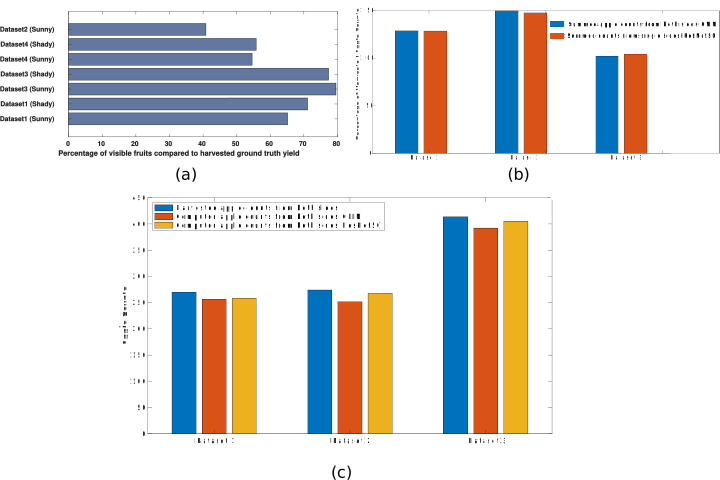
\includegraphics[width =\textwidth]{figures/map_yield/full_yield.pdf}         
        
   %\caption{An example from the GMM counting method.
  
   \caption[Fruit yield estimation - the percentage of visible fruit and single side vs both sides counts.]{Fruit yield estimation. (a) Percentage of visible fruit in captured datasets. (b) Independently summed fruit counts from individual sides lead to inconsistent estimates. (c) Merging the fruit counts from both sides, we obtain a more consistent estimate from both GMM ($91.98\%\sim94.81\%$) and ResNet50 ($95.56\%\sim97.83\%$) based counting methods.}
    \label{fig:bothsideyield}
\end{figure} 

With the help of depth sensors and the unsupervised clustering based counting algorithm our system is also capable of extracting fruit diameters. In Fig.~\ref{fig:diam}, we show the measurements for the apple grades on left, our predicted fruit diameter distribution two weeks before harvest (top right) and the ground truth diameter distribution. This data was obtained from Pine Tree Orchard at Bear Lake, Minnesota.

\begin{figure}[!hbpt]

        \centering     
        
            \includegraphics[width =\textwidth]{figures/map_yield/AppleYieldEstimationOverview.pdf}         
        
   %\caption{An example from the GMM counting method.
  
   \caption[Fruit diameter estimation.]{Fruit diameter estimation. With the help of depth sensors and the unsupervised clustering based counting algorithm our system is capable of extracting fruit diameters. Here, we show the measurements for the apple grades on left, our predicted fruit diameter distribution two weeks before harvest (top right) and the ground truth diameter distribution. This data was obtained from Pine Tree Orchard at Bear Lake, Minnesota.}
    \label{fig:diam}
\end{figure} 
\section{Experimental Insights and Conclusion}\label{sec:track_conc}
In this chapter, we presented methods for combining fruit detection, counting and tracking techniques to obtain aggregate fruit count for the captured portion of a tree row. Our segmentation method based on semi-supervised clustering combined with the Convolutional Neural Network (CNN) based counting approach from H{\"a}ni et. al.~\cite{hani_jfr_counting}, achieved state-of-the-art yield accuracies ranging from $95.56\%-97.83\%$ outperforming all existing methods. When equipped with depth cameras, by using the unsupervised counting method the system is also capable of extracting fruit size.

One of the main takeaways from our conducted experiments is that the number of visible fruit from a single side of a row varies a lot from datasets to datasets ($40.85\% - 79.83\%$) (See Fig.~\ref{fig:bothsideyield}(a)). To obtain a consistent estimate of fruit count thus it is essential to have a coherent geometric representation of the entire tree row from both sides. Apart from yield estimation, the merged reconstructions are also useful for measuring several geometric traits such as - canopy volume, trunk diameter, and tree heights.

A weakness of our system, in contrast to other state-of-the-art yield mapping methods~\cite{wang,sa_deepfruits:_2016,bargoti_deep_2017,stein_image_2016} is that it does not have a consistent estimator of fruit that is not visible in the captured footage. Despite we achieved high accuracy as in our experimental settings most of the fruit was visible from at least one side of the row. To ensure good performance in settings, where most of the fruit is not visible, our system needs to be augmented with additional predictive algorithms.


This brings us to the end of the first part of this dissertation which was dedicated to developing practical solutions for yield mapping. We presented a flexible framework where different units have integrated in a modular way so that any of them can be changed without affecting others. In the next chapter, we move to the second part where we study view planning strategies for a mobile manipulator charged with counting fruit accurately.   

